\documentclass[11pt, oneside]{article}   	% use "amsart" instead of "article" for AMSLaTeX format
\usepackage[margin = 1in]{geometry}                		% See geometry.pdf to learn the layout options. There are lots.
\geometry{letterpaper}                   		% ... or a4paper or a5paper or ... 
%\geometry{landscape}                		% Activate for rotated page geometry
\usepackage[parfill]{parskip}    		% Activate to begin paragraphs with an empty line rather than an indent
\usepackage{graphicx}				% Use pdf, png, jpg, or eps§ with pdflatex; use eps in DVI mode
								% TeX will automatically convert eps --> pdf in pdflatex		
\usepackage{amssymb, enumerate, tikz, multicol}

%SetFonts

%SetFonts


\title{Math F113X: Homework Set 6}
%\author{The Author}
\date{}							% Activate to display a given date or no date

\begin{document}

\maketitle

\vspace{-1.5cm}


\fbox{\parbox{\textwidth}{

\begin{itemize}
\item Start with the Problems A and B on minimum cost spanning trees.
\item Then complete the \emph{introductory problem} on Euler circuits and paths, Problem C.
\item Last, complete the problems from the Graph Theory  section:
\begin{quote}\# 1, 13,14,15,16, 30, 32, 35a \end{quote}

\item Answer the following {\bf reflection question}: What did you learn from checking your homework answers against the provided solutions?
\end{itemize}
}}
\textbf{Problem A:} Use the drawing of Graph A (in box) to answer the questions. \\
\fbox{
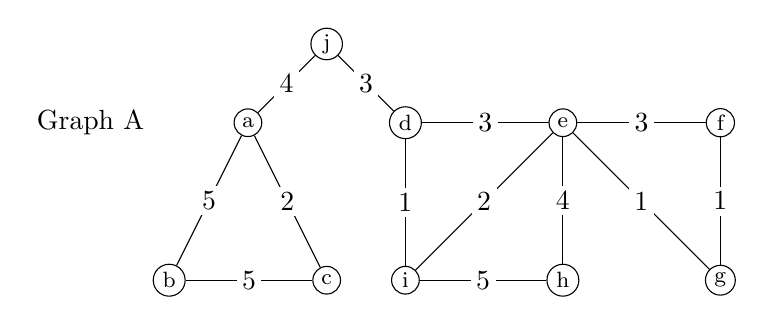
\begin{tikzpicture}[scale=1]
\node at (-1,2){Graph A};
\tikzstyle{vtx}=[circle, draw, fill=black!0,
                        inner sep=1.5pt, minimum width=10pt, font = \footnotesize]
 \tikzstyle{lbl}=[midway, inner sep = 2 pt, fill = white]                   
\node[vtx](a) at (1,2){a};
\node[vtx](b) at (0,0){b};
\node[vtx](c) at (2,0){c};
\node[vtx](d) at (3,2){d};
\node[vtx](e) at (5,2){e};
\node[vtx](f) at (7,2){f};
\node[vtx](g) at (7,0){g};
\node[vtx](h) at (5,0){h};
\node[vtx](i) at (3,0){i};
\node[vtx](j) at (2,3){j};
\foreach \i/\j/\k in {a/b/5,a/c/2,b/c/5,a/j/4,d/j/3,d/i/1,d/e/3, e/i/2,i/h/5,e/h/4,e/f/3,e/g/1,f/g/1}{\draw (\i) -- node[lbl]{\k} (\j);}
\end{tikzpicture}
}
\begin{enumerate}
\item Draw two different spanning trees of Graph A.
\item Determine the total weight of each tree from part 1 above. 
\end{enumerate}



\textbf{Problem B:} Use Kruskal's Algorithm to find a minimum cost spanning tree in each graph below. Make sure to show appropriate work.\\
\begin{multicols}{2}
Graph $B_1$\\
\fbox{
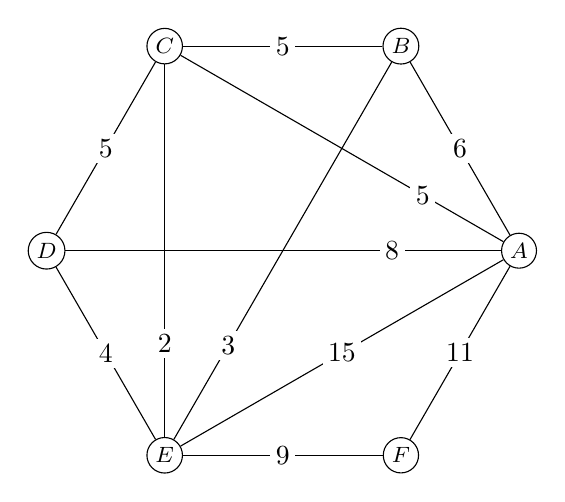
\begin{tikzpicture}
\tikzstyle{vtx}=[circle, draw, fill=black!0,
                        inner sep=1.5pt, minimum width=10pt, font = \footnotesize]
 \tikzstyle{lbl}=[midway, inner sep = 2 pt, fill = white] 
 \tikzstyle{lbb}=[pos=0.25, inner sep = 2 pt, fill = white]
	\node[vtx] (A) at (0:3){$A$};
	\node[vtx] (B) at (60:3){$B$};
	\node[vtx] (C) at (120:3){$C$};
	\node[vtx] (D) at (180:3){$D$};
	\node[vtx] (E) at (240:3){$E$};
	\node[vtx] (F) at (300:3){$F$};
	
\foreach \i/\j/\k in {A/B/6,A/E/15,B/C/5,C/D/5,D/E/4,E/F/9,A/F/11}{\draw (\i) -- node[lbl]{\k} (\j);}
\foreach \i/\j/\k in {E/C/2,A/D/8,A/C/5,E/B/3}{\draw (\i) -- node[lbb]{\k} (\j);}

\end{tikzpicture}
}

\columnbreak
Graph $B_2$\\
\fbox{
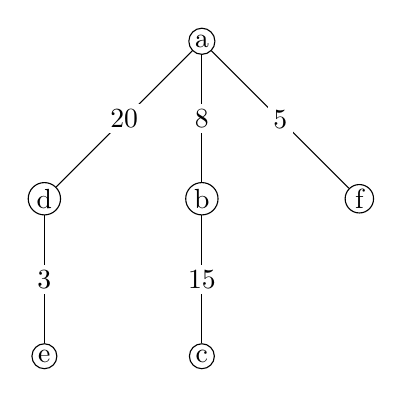
\begin{tikzpicture}
\node[draw,circle, inner sep=1pt](a) at (0,4){a};
\node[draw,circle, inner sep=1pt](b) at (0,2){b};
\node[draw,circle, inner sep=1pt](d) at (-2,2){d};
\node[draw,circle, inner sep=1pt](f) at (2,2){f};
\node[draw,circle, inner sep=1pt](c) at (0,0){c};
\node[draw,circle, inner sep=1pt](e) at (-2,0){e};
 \tikzstyle{lbl}=[midway, inner sep = 2 pt, fill = white]
 \foreach \i/\j/\k in {a/d/20,a/b/8,a/f/5,d/e/3,b/c/15}{\draw (\i) -- node[lbl]{\k} (\j);}
\end{tikzpicture}
}
\end{multicols}

\textbf{Problem C:} For each graph below, determine if it has an Euler circuit, an Euler path, or neither. Justify your answer. Note that you do not need to \emph{find} the Euler circuit or path, only need to determine whether it exists. \\

\begin{multicols}{3}
Graph $B_1$\\
\fbox{
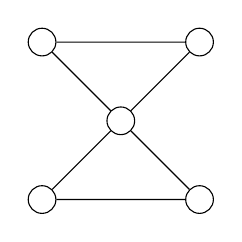
\begin{tikzpicture}
\tikzstyle{vtx}=[circle, draw, fill=black!0,
                        inner sep=1.5pt, minimum width=10pt, font = \footnotesize]
	\node[vtx] (A) at (-1,1){};
	\node[vtx] (B) at (1,1){};
	\node[vtx] (C) at (0,0){};
	\node[vtx] (D) at (-1,-1){};
	\node[vtx] (E) at (1,-1){};
\draw (A)--(B)--(C)--(D)--(E)--(C)--(A);
\end{tikzpicture}
}

\columnbreak

Graph $B_2$\\
\fbox{
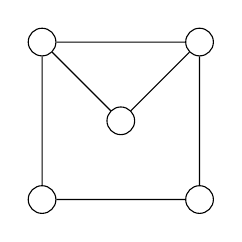
\begin{tikzpicture}
\tikzstyle{vtx}=[circle, draw, fill=black!0,
                        inner sep=1.5pt, minimum width=10pt, font = \footnotesize]
	\node[vtx] (A) at (-1,1){};
	\node[vtx] (B) at (1,1){};
	\node[vtx] (C) at (0,0){};
	\node[vtx] (D) at (-1,-1){};
	\node[vtx] (E) at (1,-1){};
\draw (A)--(B)--(C)(B)--(E)--(D)--(A)--(C);
\end{tikzpicture}
}
\columnbreak

Graph $B_3$\\
\fbox{
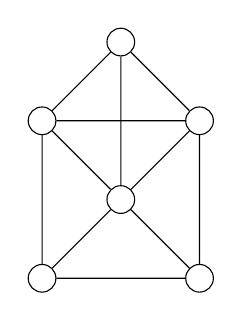
\begin{tikzpicture}
\tikzstyle{vtx}=[circle, draw, fill=black!0,
                        inner sep=1.5pt, minimum width=10pt, font = \footnotesize]
	\node[vtx] (A) at (-1,1){};
	\node[vtx] (B) at (1,1){};
	\node[vtx] (C) at (0,0){};
	\node[vtx] (D) at (-1,-1){};
	\node[vtx] (E) at (1,-1){};
	\node[vtx] (f) at (0,2){};
\draw (A)--(B)--(C)--(D)--(E)--(C)--(A)--(D)(E)--(B);
\draw (A)--(f)--(B)(C)--(f);
\end{tikzpicture}
}
\end{multicols}


\hrulefill

Remember to write up your homework solutions according to the homework writeup guidelines. 

Homework is graded using the following rubric for each problem (or problem part):

\begin{description}
\item[2 points:] You provided a complete answer, with supporting work, written up clearly
\item[1 point:] Some attempt at a solution, but incomplete writeup / unclear / illegible / no answer
\item[1 point:] Only an answer, with no supporting work 
\item[0 points:] Missing.
\end{description}

After you do the homework, you need to check your answers against the solutions! Then figure out your errors (if any) and revise your homework before you submit it. Finally, answer the reflection question.

Homework must be submitted on Gradescope.

\end{document}  